\chapter{Implementation and Evaluation}

%-------------------------------------------------------------
\section{Introduction}
%-------------------------------------------------------------

This chapter presents the technical environment of Ask-Jade and evaluates
the performance of the final system. The evaluation relies on the
LLM-as-a-Judge paradigm, with all metrics tracked through Langfuse.
Results are analysed both for the initial architecture (vector retrieval
combined with a Neo4j knowledge graph) and the final architecture
(vector-only retrieval), in order to justify the removal of the graph
component.

%-------------------------------------------------------------
\section{Technical Specification}
%-------------------------------------------------------------

\subsection{Hardware Environment}

The system was developed and tested on the two machines described in
Table \textbf{5.1}.

\begin{table}[H]
\centering
\caption{Hardware Environment}
\label{tab:hardware}
\begin{tabular}{|l|c|c|}
\hline
\textbf{Component} & \textbf{HP Pavilion x360} & \textbf{ASUS V16} \\
\hline
CPU     & Intel Core i5 (8\textsuperscript{th} Gen)
        & Intel Core i7 (13\textsuperscript{th} Gen) \\
\hline
RAM     & 9 GB   & 24 GB \\
\hline
GPU     & NVIDIA GeForce & NVIDIA RTX 4050 \\
\hline
Storage & 1 TB HDD & 500 GB SSD \\
\hline
\end{tabular}
\end{table}

%-------------------------------------------------------------
\subsection{Software Environment}
%-------------------------------------------------------------

Table \textbf{5.2} presents the main software tools used in the project.

\setlength{\LTleft}{\fill}
\setlength{\LTright}{\fill}
\renewcommand{\arraystretch}{1.4}

\begin{longtable}{|>{\centering\arraybackslash}m{3cm}
                   |>{\RaggedRight\arraybackslash}p{10cm}|}

  \caption{Software Environment}
  \label{tab:software} \\
  \hline
  \textbf{Software} & \textbf{Description} \\
  \hline
  \endfirsthead
  \hline
  \textbf{Software} & \textbf{Description} \\
  \hline
  \endhead
  \hline
  \endfoot
  \hline
  \endlastfoot

  \raisebox{-0.5\height}{
\includegraphics[height=1.1cm]{vscode_logo.png}}
  &
  \textbf{Visual Studio Code}~\cite{vscode} is a lightweight source-code
  editor available on Windows, Linux, and macOS, used for all development
  tasks in this project.
  \\ \hline

  \raisebox{-0.5\height}{
\includegraphics[height=1.1cm]{python_logo.png}}
  &
  \textbf{Python 3.11}~\cite{python} is the main programming language of the
  Ask-Jade backend, chosen for its rich AI/ML ecosystem including LlamaIndex,
  sentence-transformers, and FastAPI.
  \\ \hline

  \raisebox{-0.5\height}{
\includegraphics[height=1.1cm]{github_logo.png}}
  &
  \textbf{GitHub}~\cite{github} is the version-control platform used for
  code hosting, branch management, and CI/CD automation throughout the
  project.
  \\ \hline

  \raisebox{-0.5\height}{
\includegraphics[height=1.1cm]{postgres_logo.png}}
  &
  \textbf{PostgreSQL}~\cite{postgresql} with the \texttt{pgvector} extension
  serves as the vector database. Each document chunk is stored as a
  1{,}024-dimensional BGE-M3 embedding and retrieved using an HNSW index.
  \\ \hline

  \raisebox{-0.5\height}{
\includegraphics[height=1.1cm]{langfuse_logo.png}}
  &
  \textbf{Langfuse}~\cite{langfuse} is an open-source LLM observability
  platform that records every generation trace and computes the
  LLM-as-a-Judge evaluation metrics described in
  Chapter~2 (Section~\ref{sec:llm_as_judge}).
  \\ \hline

\end{longtable}

%-------------------------------------------------------------
\section{System Interfaces}
\label{sec:system_interfaces}
%-------------------------------------------------------------

This section presents the main interfaces of Ask-Jade, one per use case
identified in the needs analysis.

%-------------------------------------------------------------
\subsection{Ask Questions and Manage Conversations}
%-------------------------------------------------------------

The chat interface allows users to submit natural language questions and
manage their conversation history from the same view. Each generated answer
includes source citations showing the document name, page number, and
section title. Users can create new conversations, rename or delete existing
ones, and search through their history from the left sidebar.

%-------------------------------------------------------------
\subsection{Manage Documents}
%-------------------------------------------------------------

The document management interface allows the Document Manager to upload,
archive, restore, and delete files (PDF, DOCX, PPTX).
After upload, the system processes the file and assigns it a
Pending Validation status until its metadata is reviewed.

\begin{figure}[H]
  \centering
  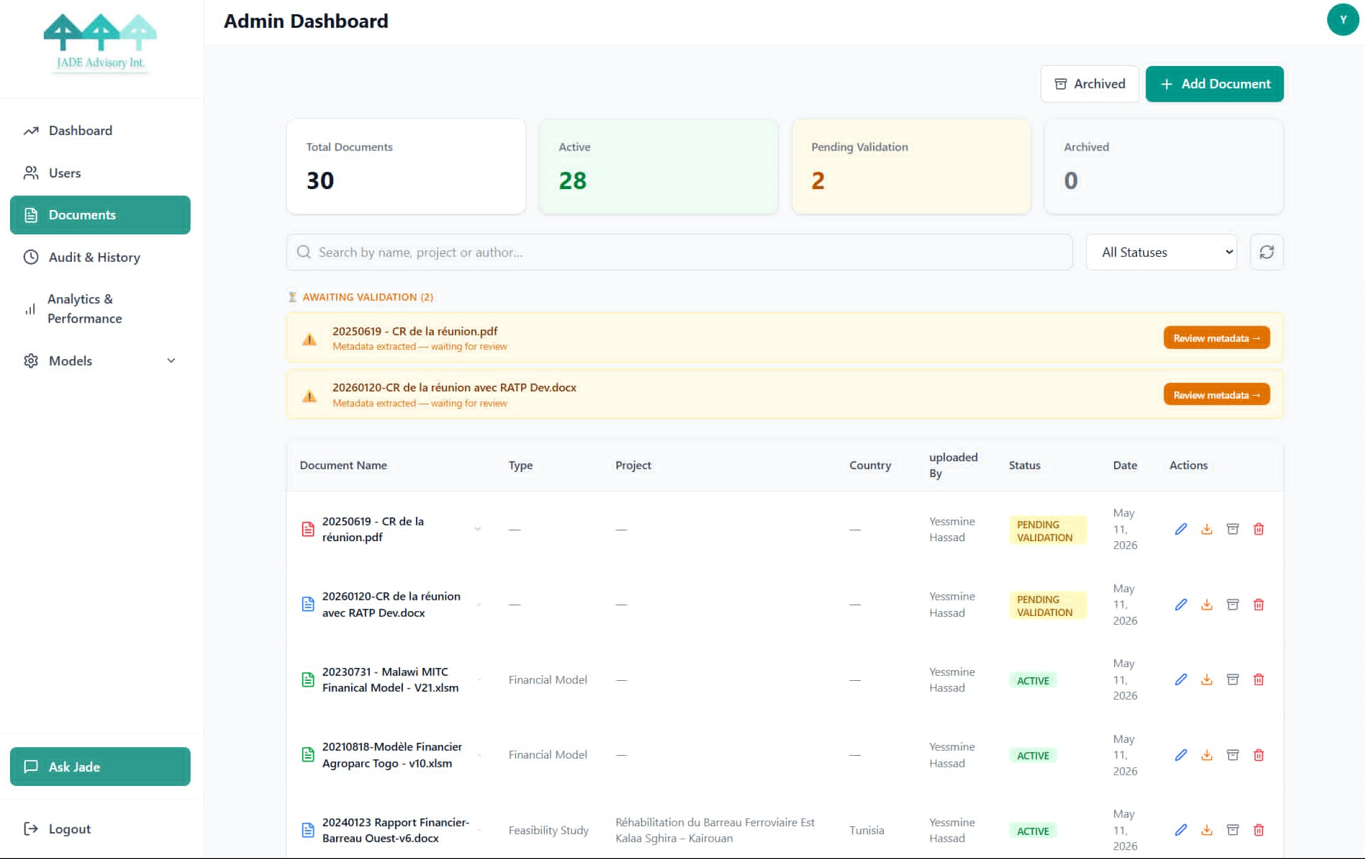
\includegraphics[width=0.95\textwidth]{document_dashboard.png}
  \caption{Document Management Interface}
  \label{fig:interface_documents_main}
\end{figure}



%-------------------------------------------------------------
\subsection{Manage Metadata}
%-------------------------------------------------------------

Triggered automatically after document upload, this interface allows the
Document Manager to review, complete, correct, and validate the metadata
extracted by Docling. Once all required fields are confirmed and a project
is associated, the document status changes to Active and becomes
searchable in the knowledge base.

%-------------------------------------------------------------
\subsection{Manage User Accounts}
%-------------------------------------------------------------

The user management interface allows the Administrator to add, edit,
archive, and delete user accounts. Users can be filtered by role or
searched by name and email. New users receive an activation email and
appear with Pending status until they complete registration.

\begin{figure}[H]
  \centering
  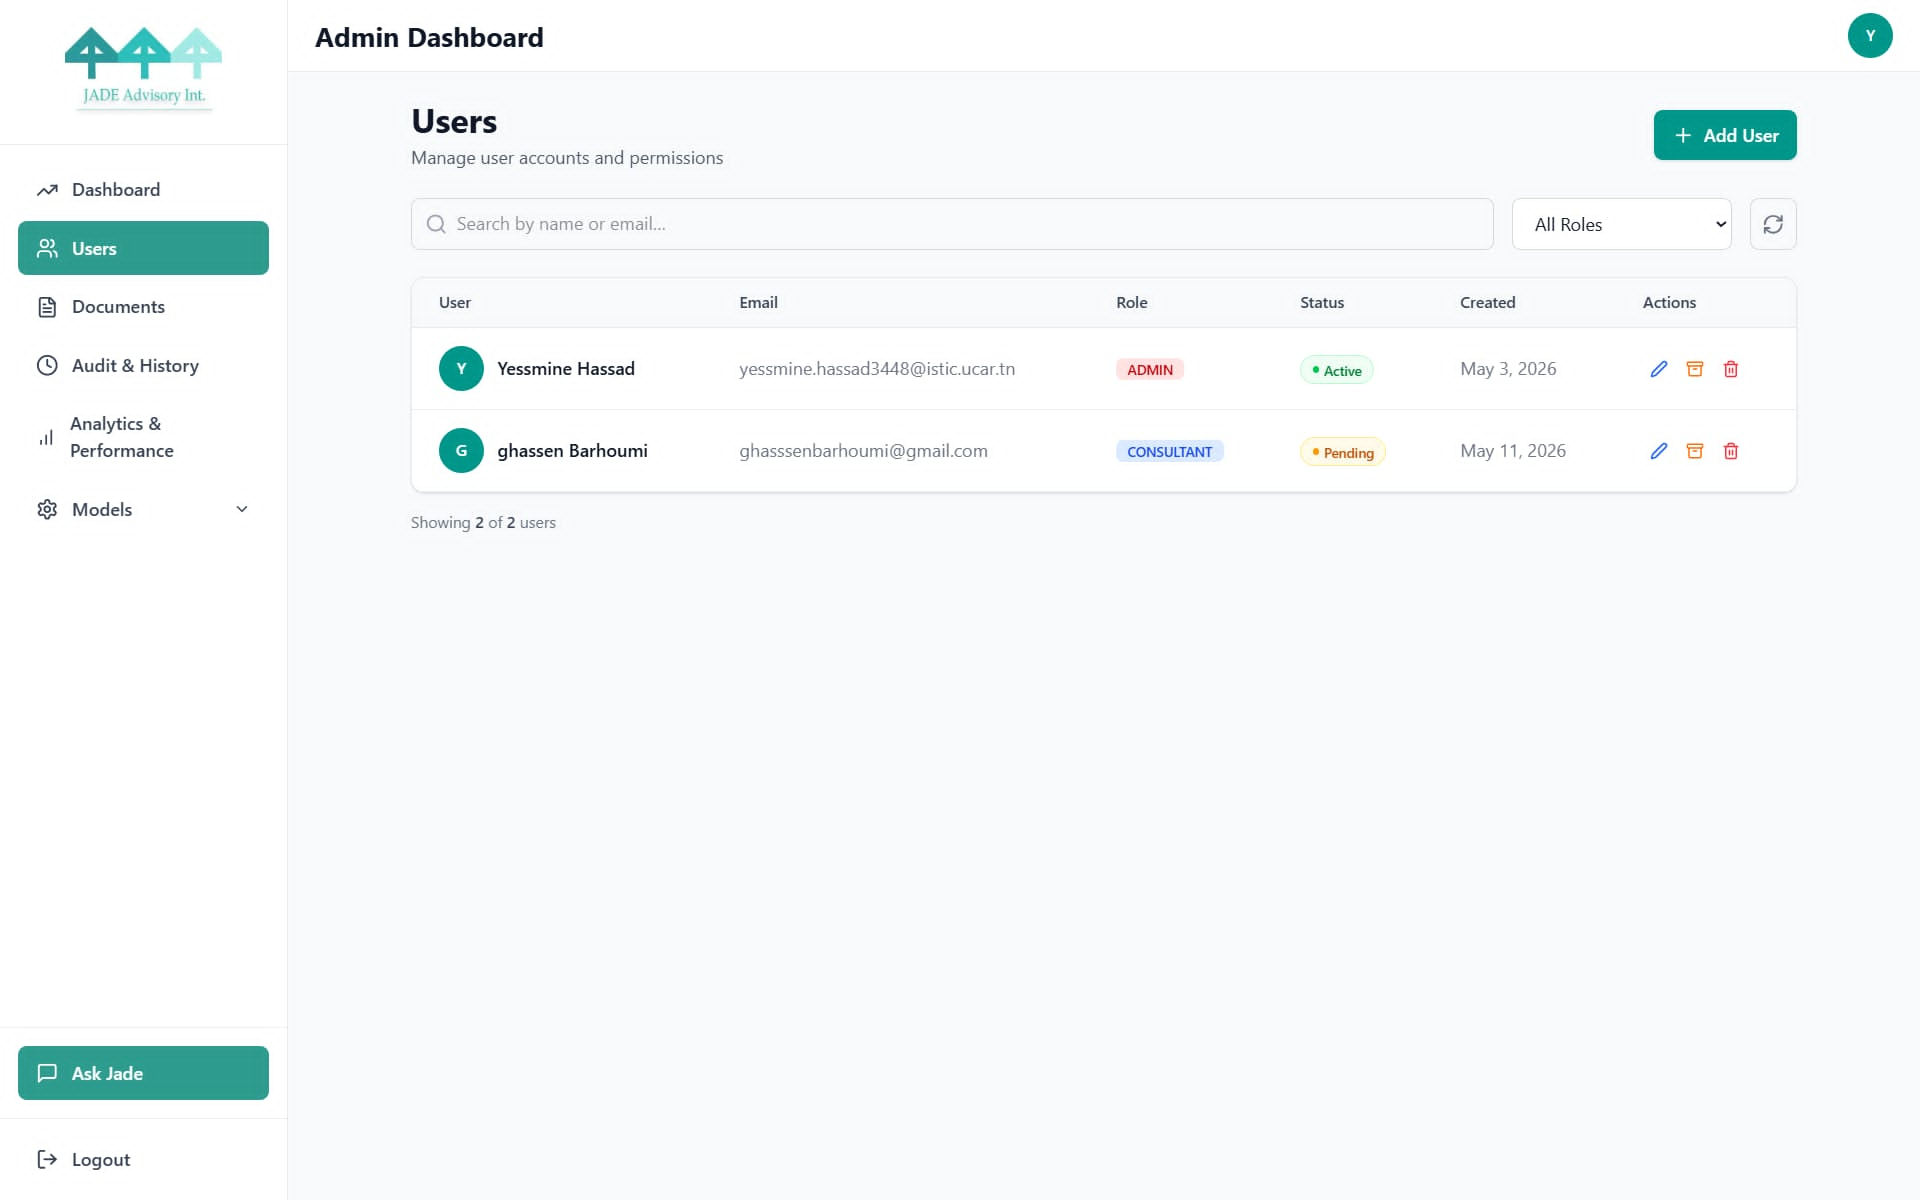
\includegraphics[width=0.95\textwidth]{users.jpg}
  \caption{User Accounts Management Interface}
  \label{fig:interface_users_main}
\end{figure}

\begin{figure}[H]
  \centering
  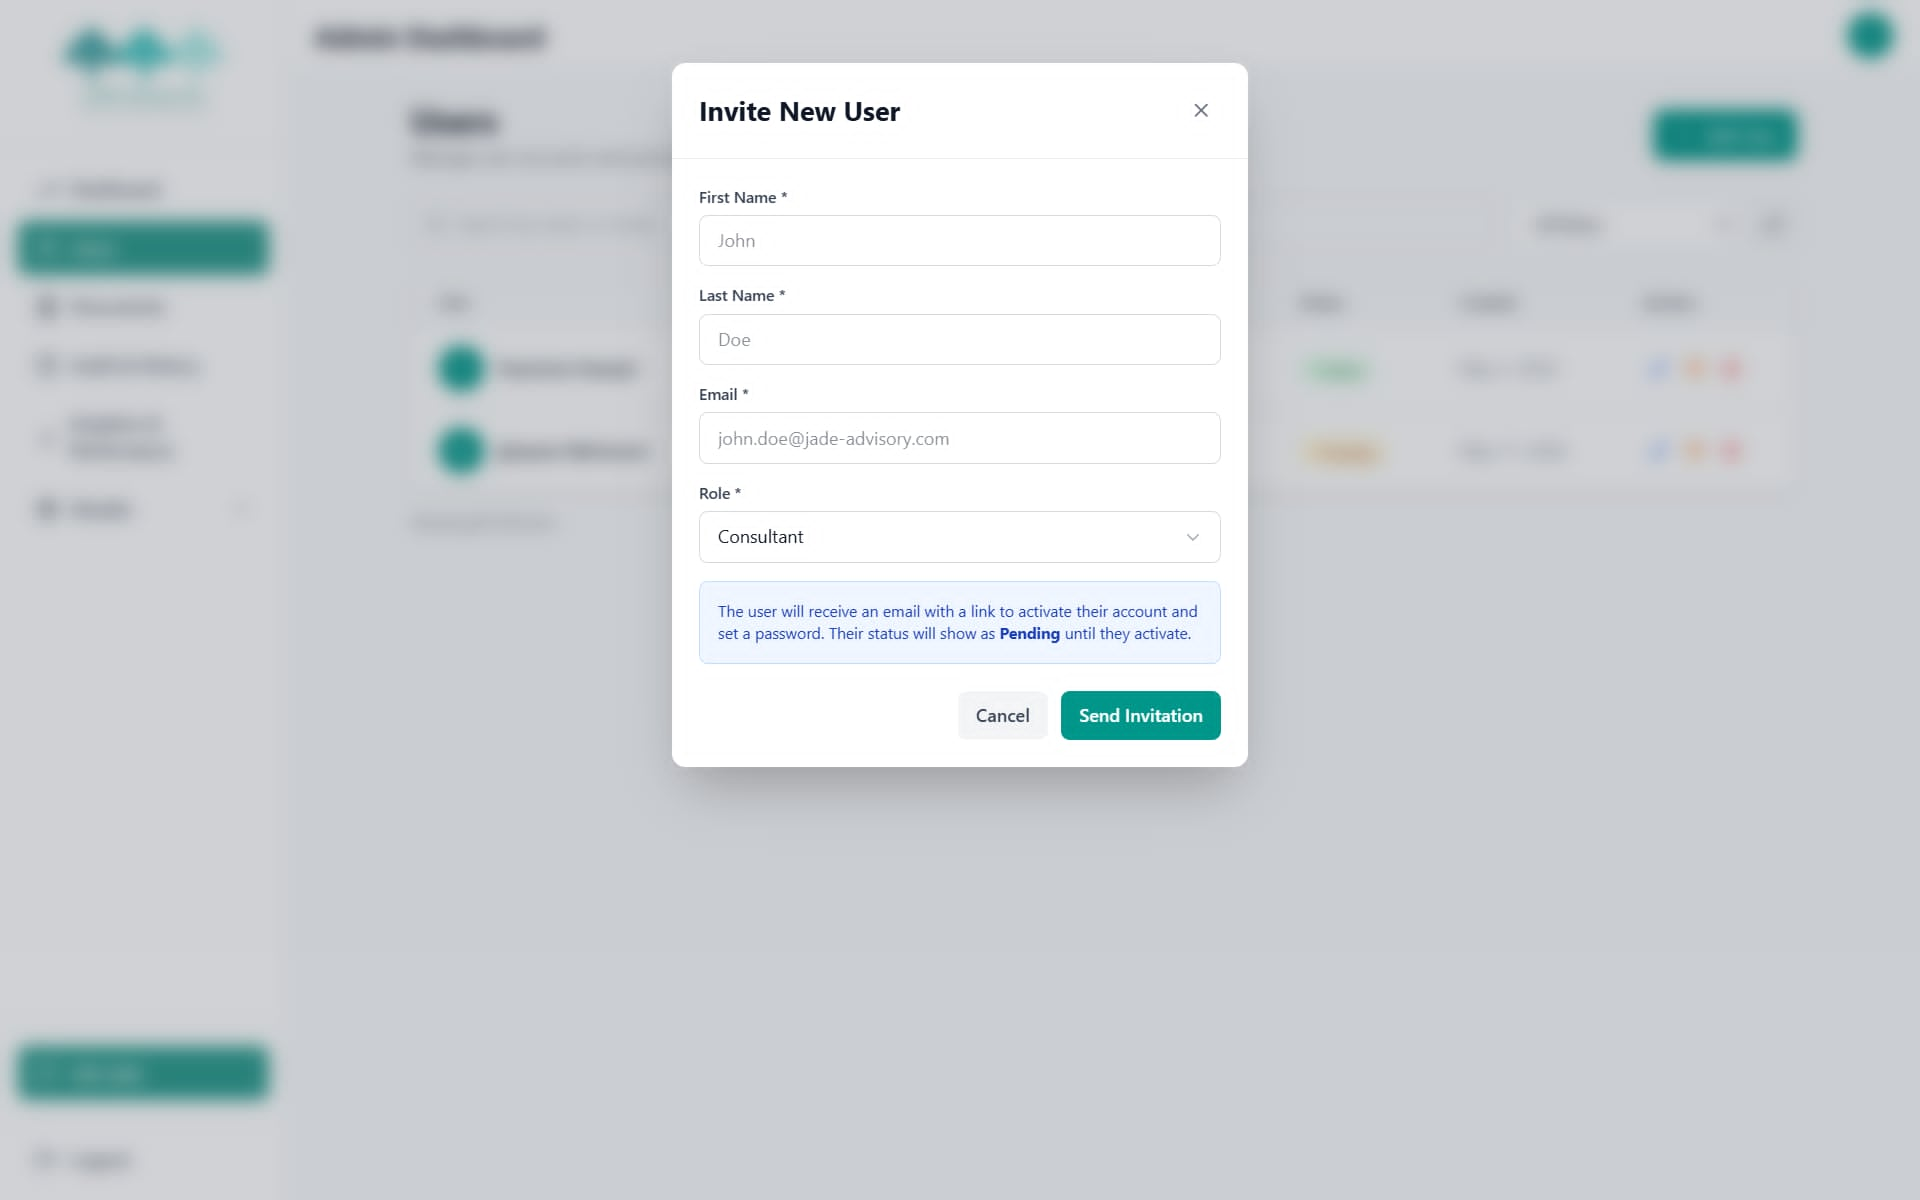
\includegraphics[width=0.75\textwidth]{invite_user.jpg}
  \caption{Invite New User Modal}
  \label{fig:interface_invite_user}
\end{figure}

%-------------------------------------------------------------
\subsection{View Logs}
%-------------------------------------------------------------

The audit logs interface provides system transparency and security
monitoring. Logs can be filtered by category (Documents, Users, System,
Security, Conversations), date range, and user, then exported in CSV
or PDF format.

%-------------------------------------------------------------
\subsection{View Questions Analytics}
%-------------------------------------------------------------

The analytics dashboard allows the Administrator to monitor system
performance, LLM usage, and evaluation metrics over configurable time
periods (7d, 30d, 90d). It displays cost, token consumption, latency
per model, and the LLM-as-a-Judge scores tracked in Langfuse.

\begin{figure}[H]
  \centering
  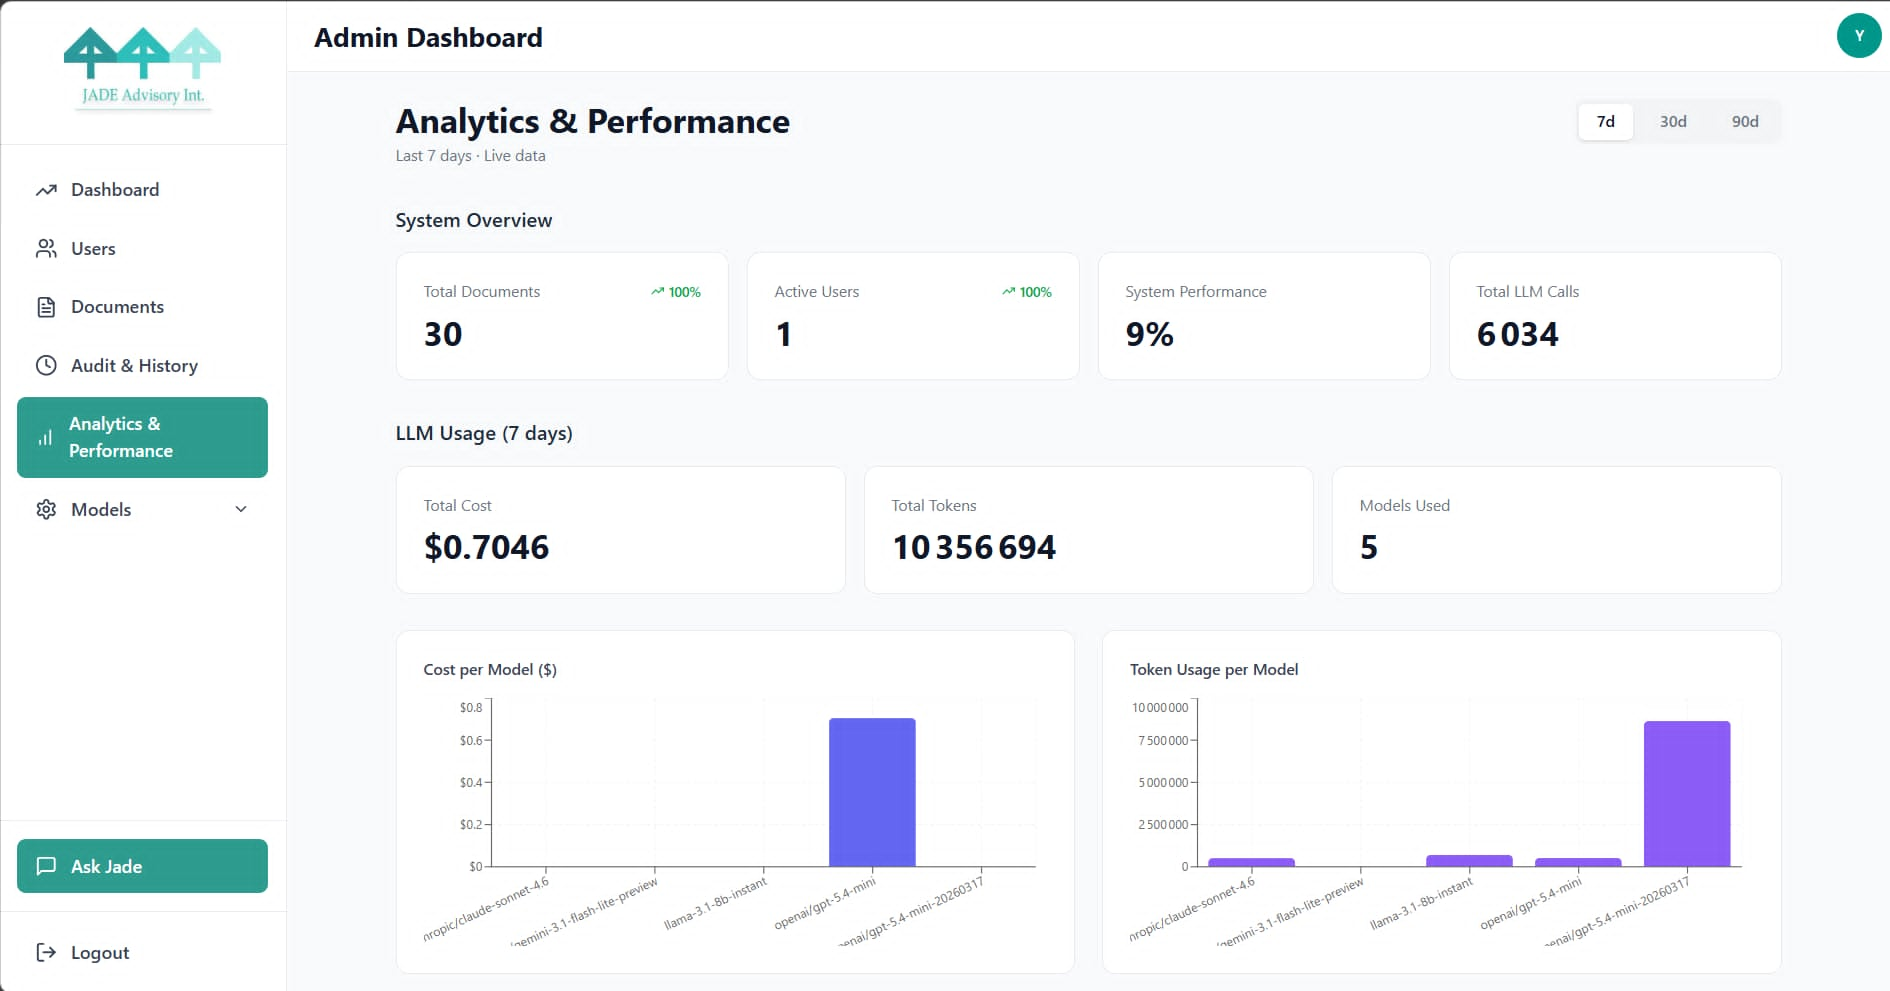
\includegraphics[width=0.95\textwidth]{performance.jpg}
  \caption{Analytics Dashboard --- System Overview and LLM Usage}
  \label{fig:interface_analytics_overview}
\end{figure}

\begin{figure}[H]
  \centering
  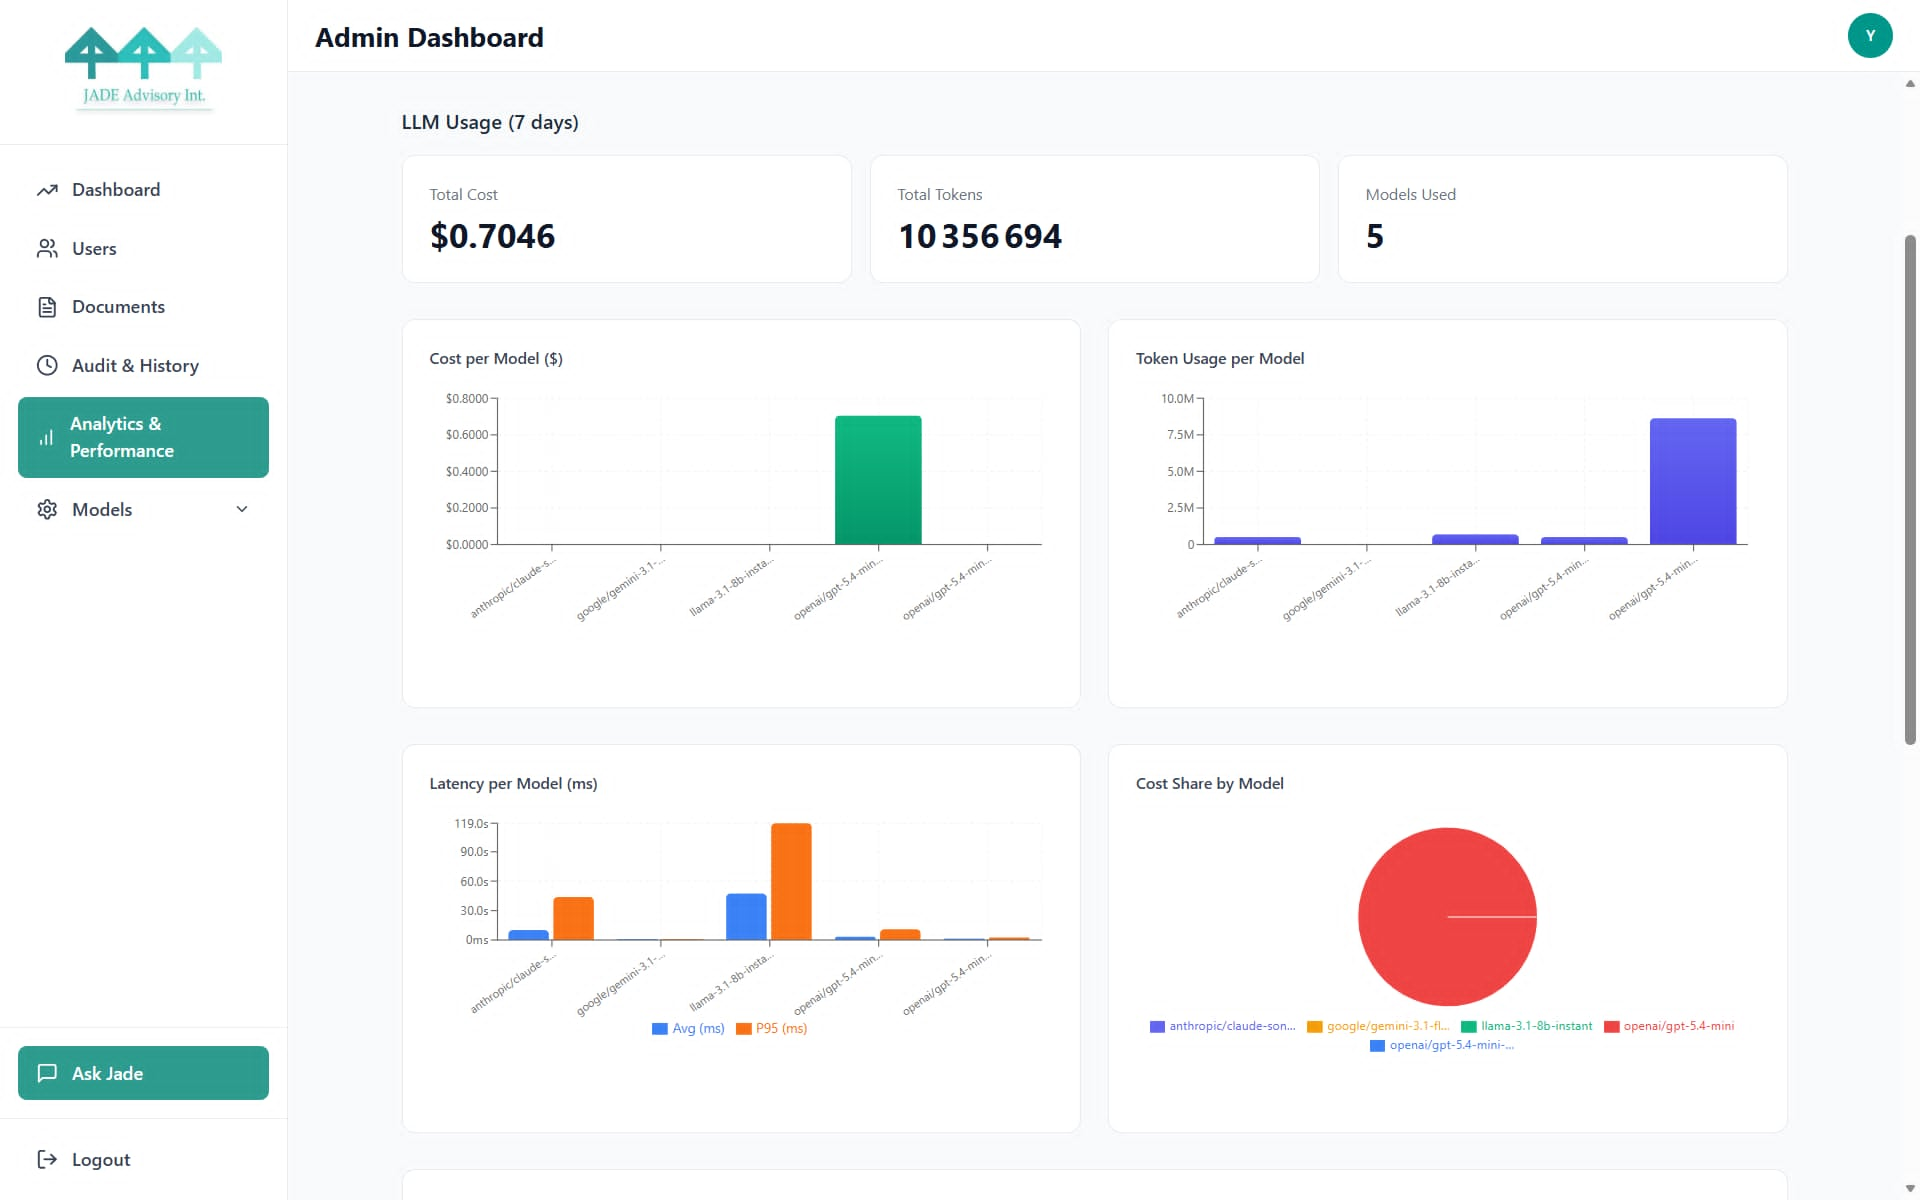
\includegraphics[width=0.95\textwidth]{analytics_scores_details.jpg}
  \caption{Model Performance and Costs}
  \label{fig:interface_analytics_costs}
\end{figure}

\begin{figure}[H]
  \centering
  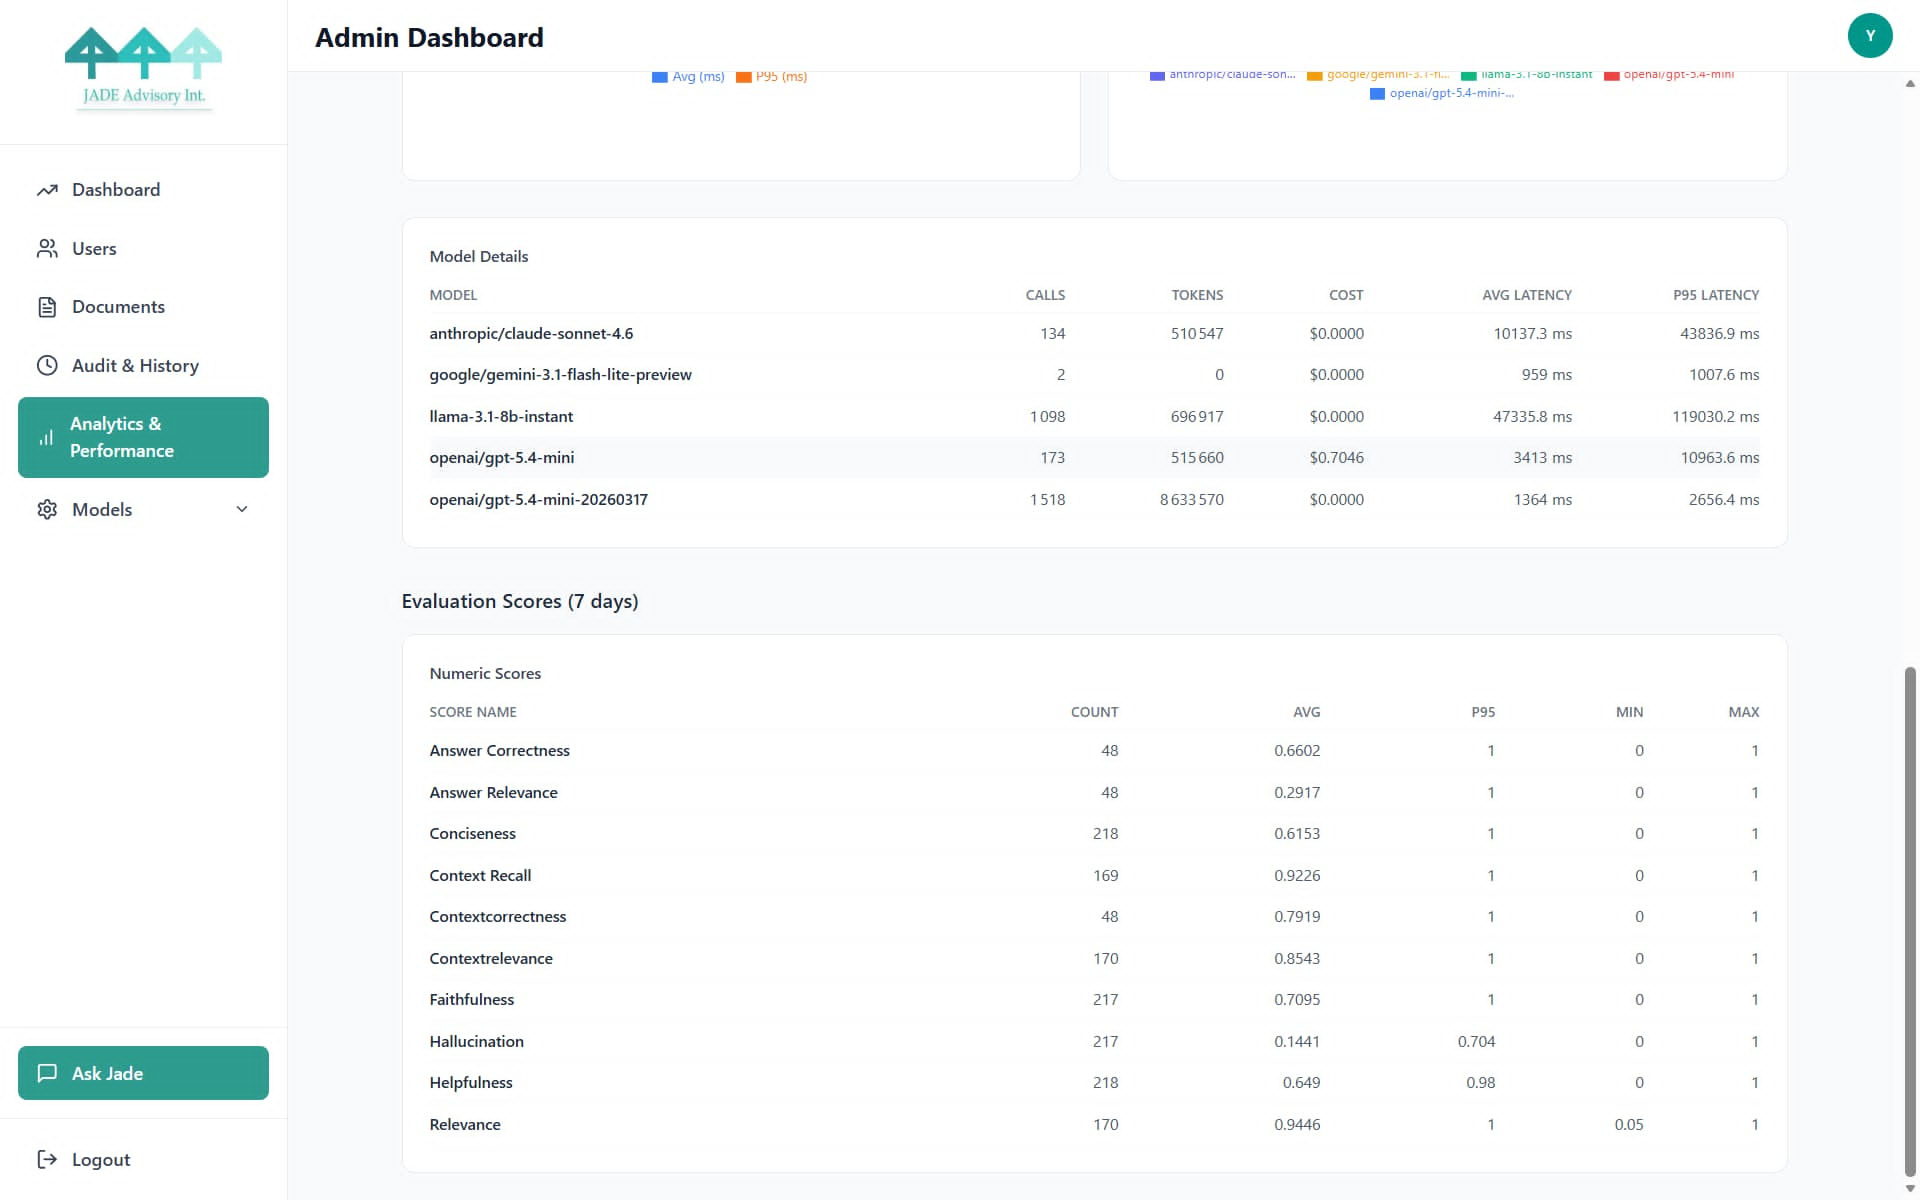
\includegraphics[width=0.95\textwidth]{analytics.jpg}
  \caption{Model Details and Evaluation Scores}
  \label{fig:interface_analytics_scores}
\end{figure}

%-------------------------------------------------------------
\subsection{Manage Models}
%-------------------------------------------------------------

The model management interface allows the Administrator to browse a
catalogue of 363 available LLMs, select up to 5 active models, and
designate one as the default. A ranking view categorised by domain
(General, Finance, Grounding) helps identify the best-performing models
before adding them to the internal catalogue.

\begin{figure}[H]
  \centering
  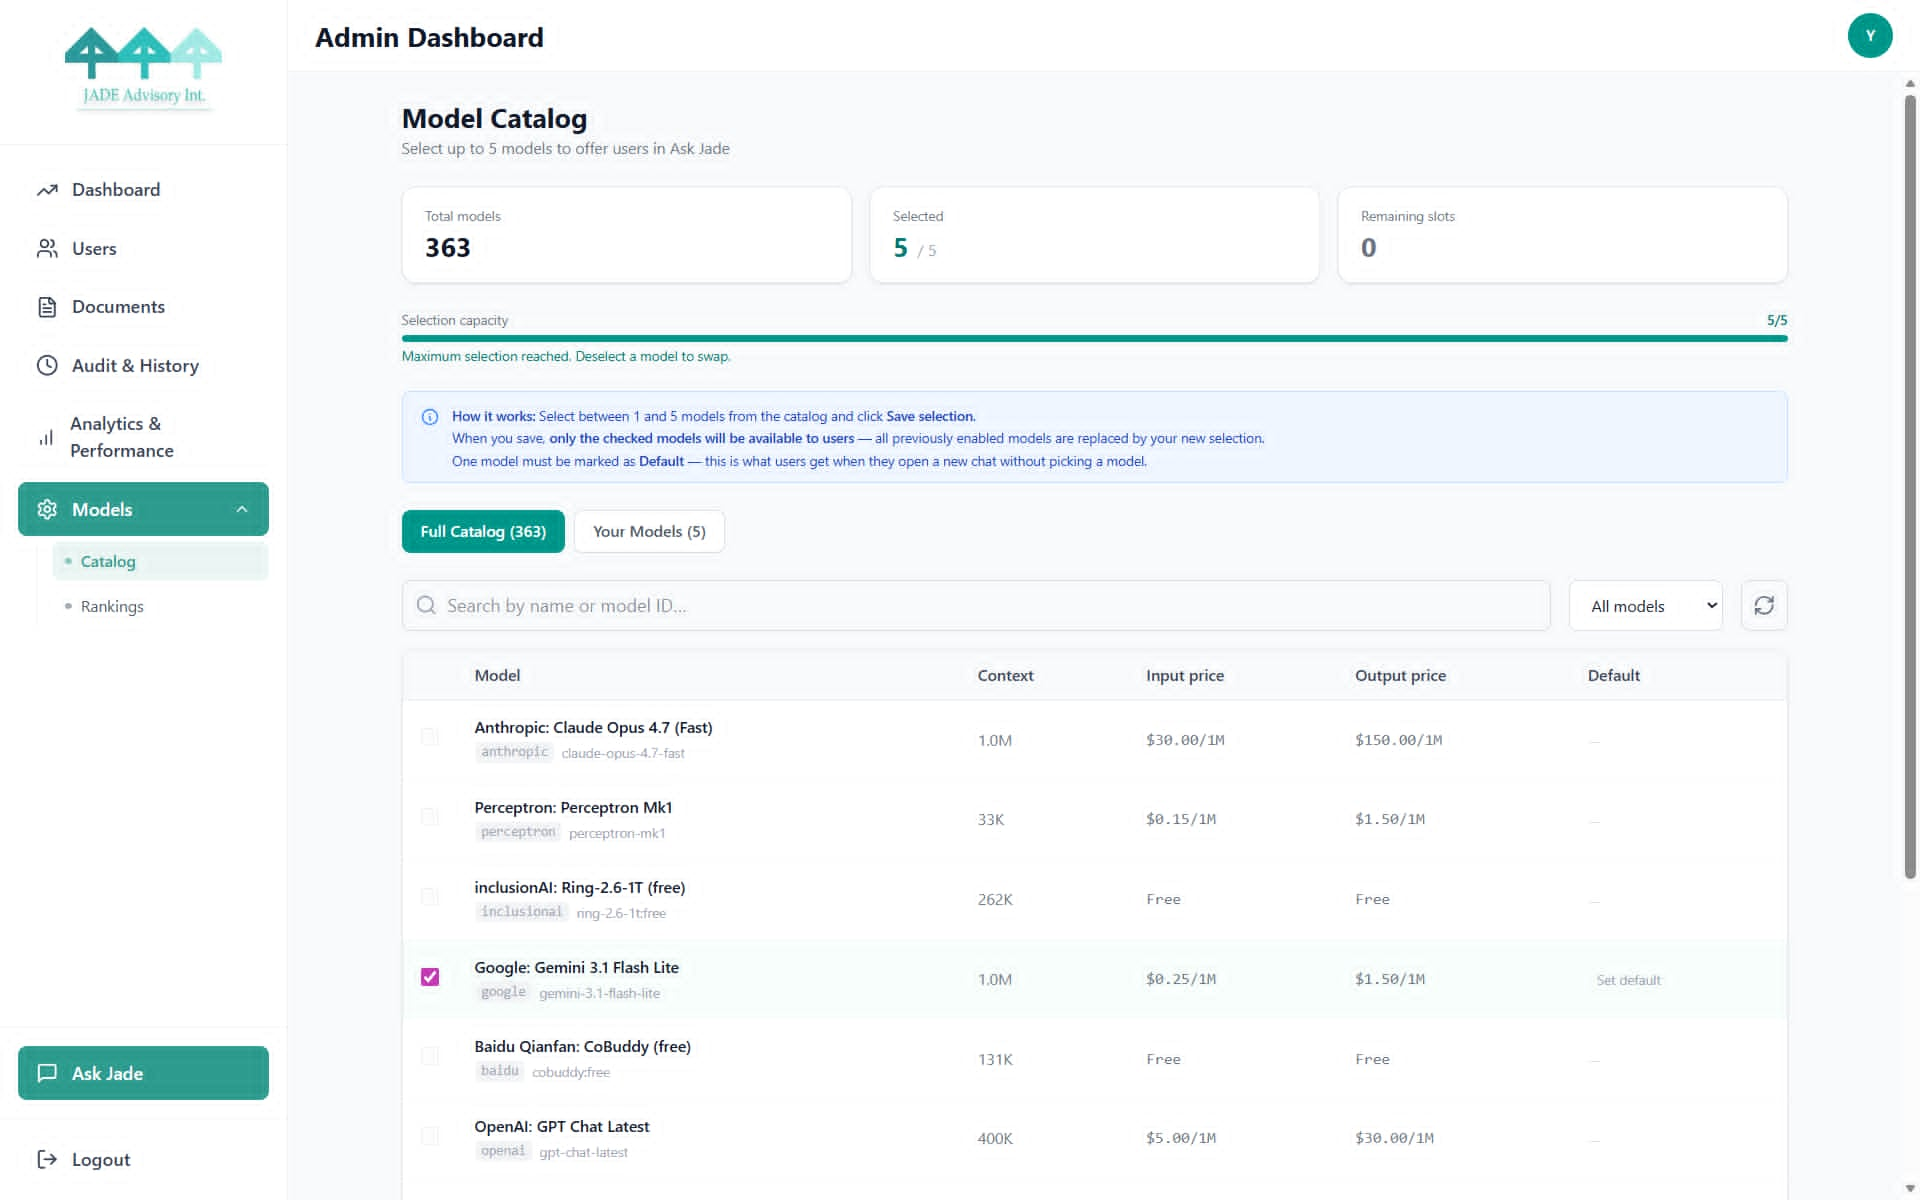
\includegraphics[width=0.95\textwidth]{catalogue.jpg}
  \caption{Model Catalog and Selection Interface}
  \label{fig:interface_models_catalog}
\end{figure}

\begin{figure}[H]
  \centering
  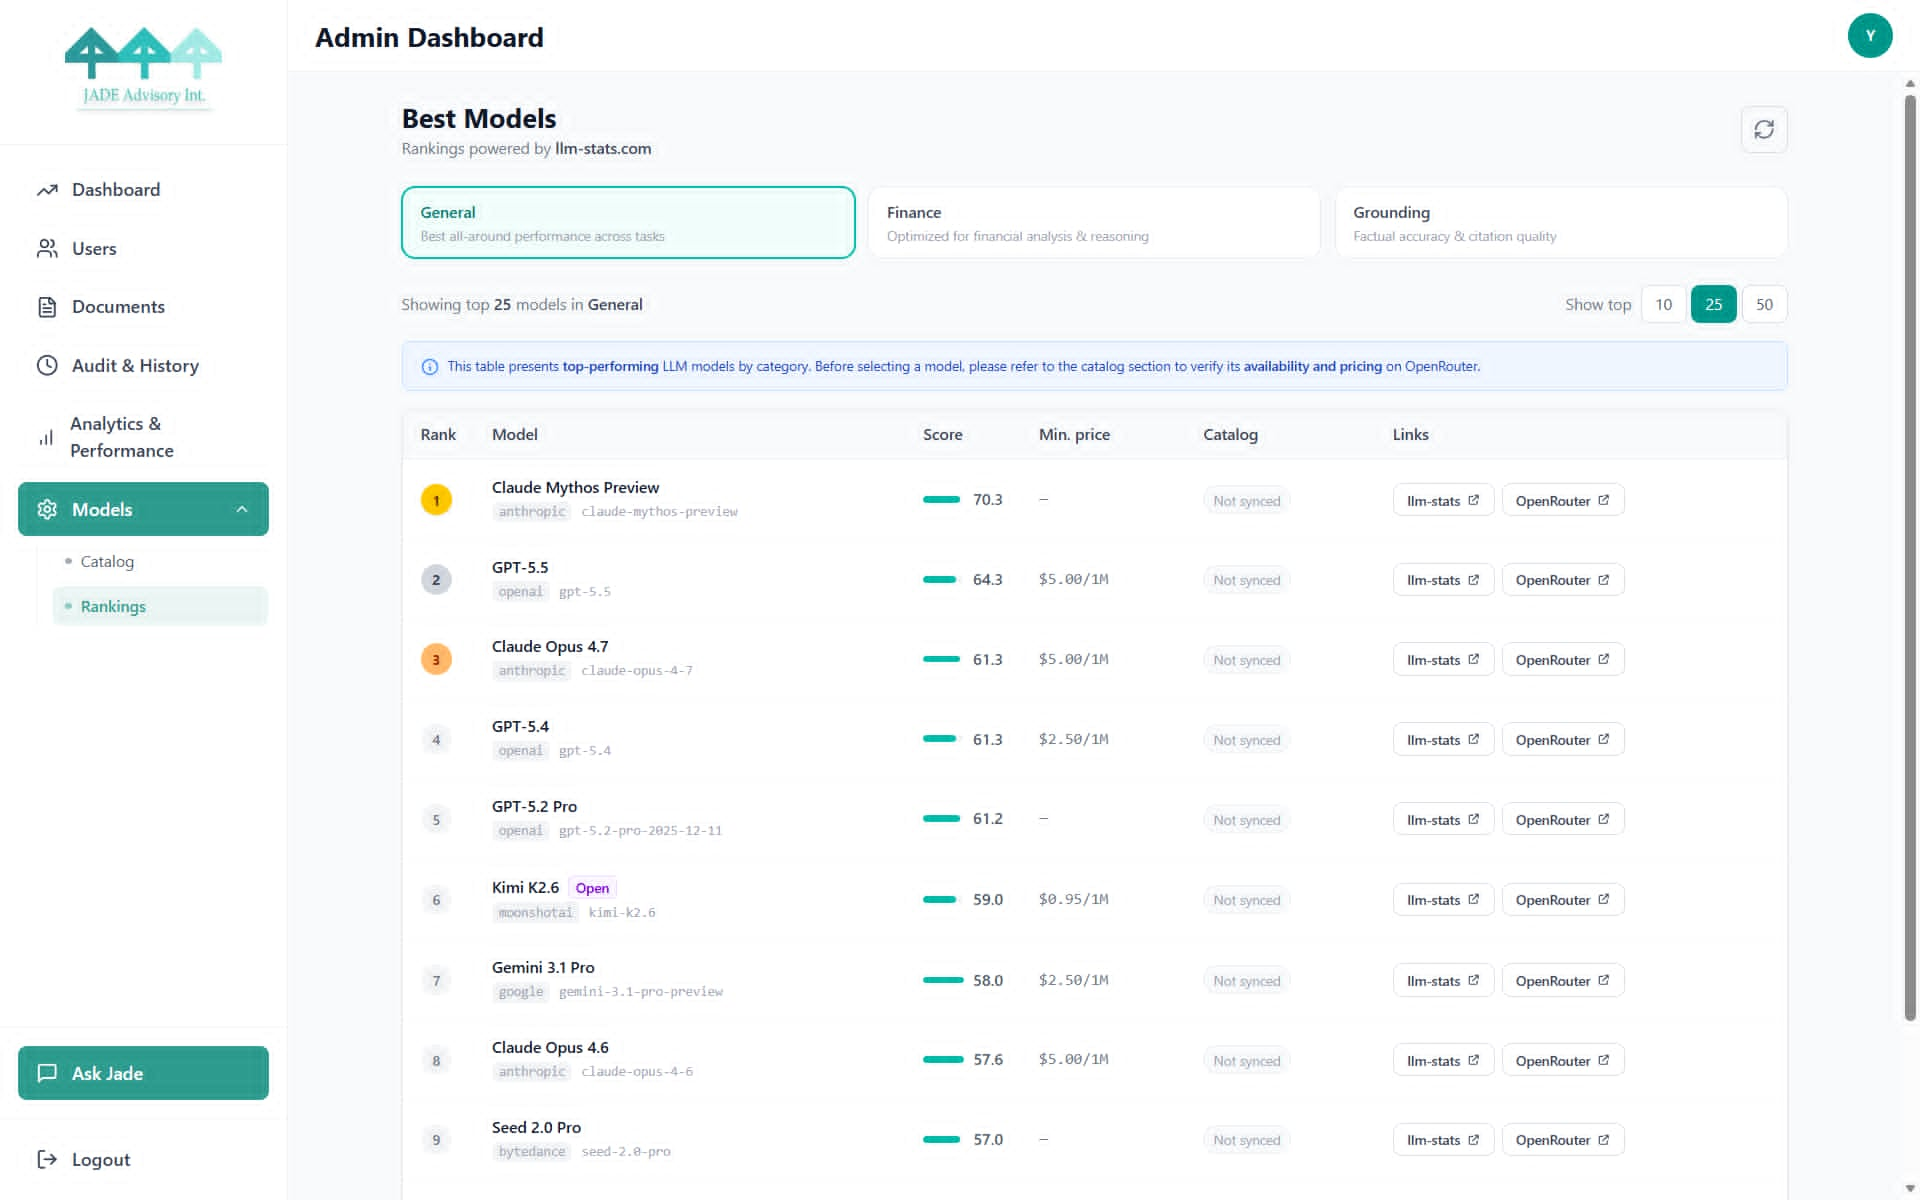
\includegraphics[width=0.85\textwidth]{rankings.jpg}
  \caption{Best Models Rankings Interface}
  \label{fig:interface_models_rankings}
\end{figure}

\begin{figure}[H]
  \centering
  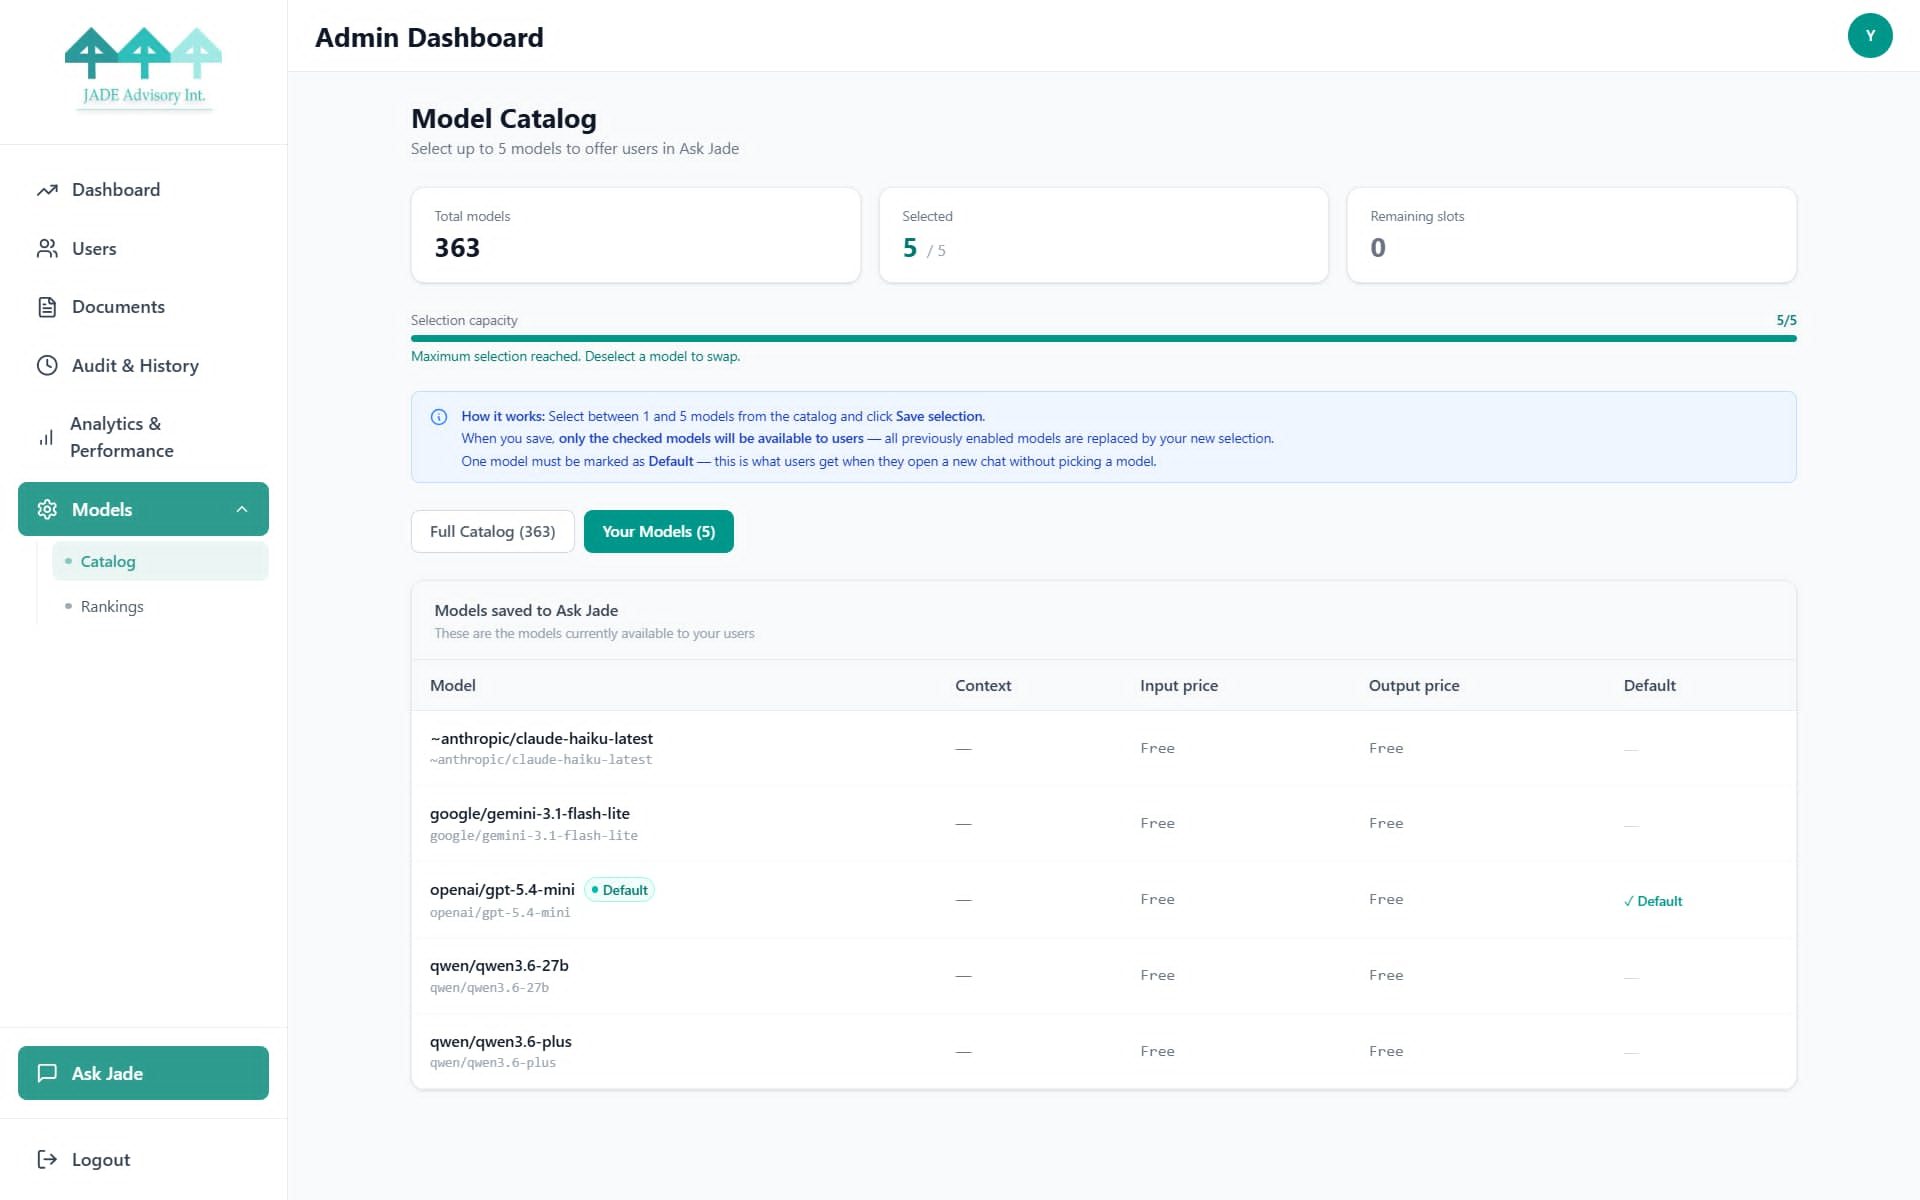
\includegraphics[width=0.85\textwidth]{your_model.jpg}
  \caption{Your Models Configuration Interface}
  \label{fig:interface_models_your_models}
\end{figure}

%-------------------------------------------------------------
\section{Evaluation Methodology}
%-------------------------------------------------------------

The evaluation of Ask-Jade relies on the LLM-as-a-Judge paradigm
presented in Chapter 2, with GPT-4o acting as the judge and all traces
logged in Langfuse. The metrics used include Context Relevance,
Context Recall, Context Correctness, Relevance, Answer Relevance,
Faithfulness, Hallucination, Answer Correctness, Helpfulness,
and Conciseness.

Two complementary approaches were used:

\begin{itemize}
  \item \textbf{Automated LLM-as-a-Judge metrics} computed over Langfuse traces during system interactions, covering retrieval and generation quality.
  \item \textbf{Human expert evaluation} based on a 27-question dataset built from Jade Advisory’s knowledge base and scored by domain experts on a 0--3 scale.
\end{itemize}

To justify the architectural decision described in the following sections, metrics were computed for two configurations:

\begin{itemize}
  \item \textbf{With graph}: vector retrieval combined with a Neo4j knowledge graph.
  \item \textbf{Without graph}: vector-only retrieval.
\end{itemize}

%-------------------------------------------------------------
\section{Evaluation Dataset}
\label{sec:eval_dataset}
%-------------------------------------------------------------
This section presents the evaluation dataset, including its design
principles, question categories, and scoring methodology.

\subsection{Design Principles}

The dataset was built to satisfy four properties:

\begin{enumerate}
  \item \textbf{Jade-specificity} questions must be answerable only
        from the proprietary knowledge base.
  \item \textbf{Testability} each question has a verifiable
        ground-truth answer.
  \item \textbf{Coverage} questions span all document types:
        terrain mission reports, financial models, scoring grids,
        meeting minutes, and benchmarking studies.
  \item \textbf{Proportionality} F.Q questions require a single
        source; A.Q questions require synthesis across at least two
        documents.
\end{enumerate}

\subsection{Dataset Composition}

The dataset contains \textbf{27 questions} across three categories
(Table~\ref{tab:dataset_composition}).

\begin{table}[H]
  \centering
  \caption{Evaluation dataset composition}
  \label{tab:dataset_composition}
  \begin{tabular}{|l|c|c|c|}
    \hline
    \textbf{Category} & \textbf{Code} & \textbf{Count} & \textbf{\%} \\
    \hline
    Factual Questions  & F.Q & 8  & 29.6\% \\
    \hline
    Analysis Questions & A.Q & 14 & 51.9\% \\
    \hline
    Excel Tool Lookups & E.T & 5  & 18.5\% \\
    \hline
    \textbf{Total} & & \textbf{27} & \textbf{100\%} \\
    \hline
  \end{tabular}
\end{table}

\subsection{Question Categories}

\subsubsection{a- Factual Questions (F.Q)}

Factual questions evaluate the ability of the system to retrieve
explicit information from a single document. Examples:
\begin{itemize}
  \item (FQ-02) What are the mandatory sections of a PPP terrain mission report?
  \item (FQ-04) How are the S and M scores defined in the pre-selection methodology?
  \item (FQ-07) Définir la trame d'évaluation de la soutenabilité budgétaire.
\end{itemize}

\subsubsection{b- Analysis Questions (A.Q)}

Analysis questions require reasoning across multiple documents to
compare information, identify relationships, and generate structured
insights. Examples:
\begin{itemize}
  \item (AQ-03) What are the most recurring failure factors in PPP projects in West Africa?
  \item (AQ-09) Comment le niveau de CAPEX influence-t-il la bancabilité d'un projet PPP?
  \item (AQ-13) What mechanisms were used to balance bankability and affordability?
\end{itemize}

\subsubsection{c- Excel Tool Lookups (E.T)}

Excel lookup questions evaluate the ability of the system to retrieve
exact numerical values from structured financial tables. Any incorrect
numerical value automatically invalidates the answer. Examples:
\begin{itemize}
  \item (ET-01) What is the total CAPEX for Project [X]?
  \item (ET-04) What are the S and M scores assigned to Project [X]?
  \item (ET-05) What tariff hypotheses are used in the financial model?
\end{itemize}

\subsection{Scoring Rubric}

Expert assessors used the four-level scoring rubric in
Table~\ref{tab:scoring_rubric}.

\begin{table}[H]
\centering
\caption{Expert evaluation scoring rubric}
\label{tab:scoring_rubric}
\renewcommand{\arraystretch}{1.4}
\begin{tabular}{|c|c|p{9cm}|}
\hline
\textbf{Score} & \textbf{Level} & \textbf{Description} \\
\hline
3 & Excellent &
Complete, accurate, well-structured, and fully grounded in the retrieved
documents with no hallucinated information. \\
\hline
2 & Good &
Mostly correct and relevant, with only minor missing details or limited
imprecision. \\
\hline
1 & Partial &
Partially correct but incomplete, overly generic, or containing minor
unsupported information. \\
\hline
0 & Fail &
Incorrect, missing, or containing hallucinated facts that contradict
the source documents. \\
\hline
\end{tabular}
\end{table}

For E.T questions, any incorrect numerical value automatically gives a
score of 0. For F.Q and A.Q questions, hallucinated statements reduce
the score depending on their severity.

%-------------------------------------------------------------
\section{Evaluation Results}
%-------------------------------------------------------------
This section presents the evaluation results obtained through automated
metrics and expert assessment, along with the impact of removing the
Neo4j knowledge graph from the final architecture.

\subsection{Automated Evaluation Results}
\label{sec:ragas_results}

The automated evaluation was done using the LLM-as-a-Judge metrics
tracked in Langfuse during real interactions with Ask-Jade.
Table~\ref{tab:results_comparison} compares the average scores obtained
with the initial architecture (vector + Neo4j graph) and the final
architecture (vector only), over 616 scores (88 interactions)
for the with-graph configuration and 12,930 scores
(1,620 interactions) for the without-graph configuration.

\begin{table}[H]
\centering
\caption{Evaluation results: with graph vs.\ without graph}
\label{tab:results_comparison}
\renewcommand{\arraystretch}{1.3}
\begin{tabular}{|l|c|c|c|c|}
\hline
\textbf{Metric} & \textbf{Category} & \textbf{With Graph} & \textbf{Without Graph} & \textbf{Target} \\
\hline
Context Relevance   & Retrieval   & 0.94 & 0.95 & $\geq 0.80$ \\
\hline
Context Recall      & Retrieval   & 0.86 & 0.60 & $\geq 0.80$ \\
\hline
Context Correctness & Retrieval   & 0.79 & ---  & $\geq 0.75$ \\
\hline
Relevance           & Generation  & 0.87 & ---  & $\geq 0.85$ \\
\hline
Answer Relevance    & Generation  & 0.29 & 0.22 & $\geq 0.80$ \\
\hline
Faithfulness        & Generation  & 0.56 & 0.05 & $\geq 0.80$ \\
\hline
Hallucination       & Generation  & 0.22 & 0.24 & $\leq 0.15$ \\
\hline
Answer Correctness  & Generation  & 0.66 & ---  & $\geq 0.75$ \\
\hline
Helpfulness         & Generation  & 0.34 & 0.01 & $\geq 0.75$ \\
\hline
Conciseness         & Generation  & 0.34 & 0.02 & $\geq 0.65$ \\
\hline
\end{tabular}
\end{table}

\subsubsection{Retrieval Performance}

Both configurations achieve a strong Context Relevance score
($0.94$ and $0.95$ respectively), confirming that the BGE-M3 +
PgVector + BGE-reranker pipeline consistently retrieves relevant
chunks from the knowledge base.

The Context Recall score drops significantly in the
without-graph configuration ($0.86 \to 0.60$). This gap is expected:
the knowledge graph contributed additional entity-level context that
helped the retrieval cover more of the information needed to answer
complex analytical questions. Without it, some required information is
not retrieved when it spans multiple documents.

\subsubsection{Generation Performance}

The most significant difference between the two configurations appears
in generation metrics. Faithfulness drops sharply from
$0.56$ to $0.05$ in the without-graph configuration, and
Helpfulness and Conciseness collapse to near zero.

These drops are partly explained by a language mismatch: the
LLM-as-a-Judge evaluation model is primarily optimised for English,
while a large portion of the Ask-Jade knowledge base is in French and
Arabic. This affects the judge's ability to verify claims and produces
artificially low faithfulness and helpfulness scores for multilingual
responses~\cite{ragas_multilingual}.

The \textbf{Hallucination} score remains above the target in both
configurations ($0.22$ and $0.24$), indicating that this is a
persistent issue independent of the graph component.

%--------------------------------------

\subsection{Abandonment of the Neo4j Knowledge Graph}
\label{sec:neo4j_removal}
This subsection explains why the Neo4j knowledge graph was removed
from the final architecture despite its initial integration.

\subsubsection{a- Initial Design}

The first version of Ask-Jade used a Neo4j knowledge graph.
It extracted entities (such as organisations, PPP projects, contracts,
and financial information) from document chunks using Gemini Flash Lite,
and stored them as nodes and relationships in the graph database.
During retrieval, results from the graph and the vector database were
combined before being sent to the language model.

\subsubsection{b- Problems Encountered}

Even though it slightly improved Context Recall, the knowledge graph
was removed from the final system for several reasons:

\begin{enumerate}
  \item \textbf{Lower answer quality.}
        Mixing graph results with vector search often added unnecessary
        information, which reduced clarity and precision.

  \item \textbf{Extraction errors.}
        Gemini Flash Lite made mistakes when extracting entities,
        especially in French and Arabic documents, which affected graph quality.

  \item \textbf{High cost.}
        Entity extraction required many extra API calls with little gain
        in performance.

  \item \textbf{Higher latency.}
        Using both graph and vector search increased response time.
\end{enumerate}

\subsubsection{c- Decision}

The results in Table~\ref{tab:results_comparison} show that the
vector-only approach performs as well or better in terms of
Context Relevance, while avoiding the issues of cost, errors,
and latency. Therefore, the final version of Ask-Jade uses only
PgVector with the BGE-reranker-v3 model. This simplified design is
faster, cheaper, and more reliable for most queries.


%-------------------------------------------------------------
\subsection{Expert Evaluation Results}
%-------------------------------------------------------------

In addition to automated evaluation, a manual assessment was conducted
by two consultants from Jade Advisory using the scoring rubric
presented in Table~\ref{tab:scoring_rubric}.